\documentclass[tikz,border=5pt]{standalone}
\usepackage{amsmath,amssymb}
\usetikzlibrary{calc}

\begin{document}
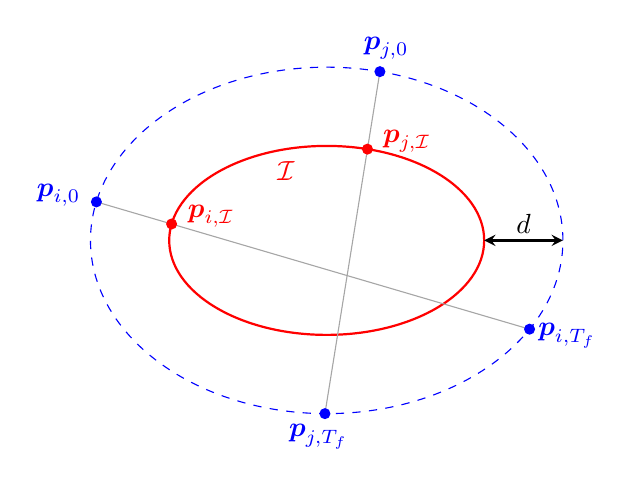
\begin{tikzpicture}[>=stealth]

  % ---------- Geometry parameters ----------
  \def\a{2.0}      % horizontal semi-axis of inner ellipse I_1
  \def\b{1.2}      % vertical   semi-axis of inner ellipse I_1
  \def\d{1.0}      % distance d between inner and outer ellipse
  \def\angi{170}   % parameter angle of the first  inner point (degrees)
  \def\angj{75}    % parameter angle of the second inner point (degrees)

  % ---------- Point names (any math-mode LaTeX, e.g. x_1, \xi, P^*, \tilde{Q}) ----------
  % First line:  inner point / outer point / opposite outer point
  \def\ptImpacti{\boldsymbol p_{i,\mathcal I}}
  \def\ptStarti{\boldsymbol p_{i,0}}
  \def\ptEndi{\boldsymbol p_{i,T_f}}
  % Second line
  \def\ptImpactj{\boldsymbol p_{j,\mathcal I}}
  \def\ptStartj{\boldsymbol p_{j,0}}
  \def\ptEndj{\boldsymbol p_{j,T_f}}

  % Outer ellipse depends on the inner one: semi-axes grow by d
  \pgfmathsetmacro{\A}{\a+\d}   % horizontal semi-axis of outer ellipse I_0
  \pgfmathsetmacro{\B}{\b+\d}   % vertical   semi-axis of outer ellipse I_0

  % ---------- Macro: draws one chord ----------
  % #1 = parameter angle of the point on the inner ellipse
  % #2, #3, #4 = names of the inner point, outer point, opposite outer point
  %              (set in math mode, so pass plain math such as P or x_1)
  \newcommand{\chord}[4]{%
    \begin{scope}
      % Point on the inner ellipse
      \pgfmathsetmacro{\px}{\a*cos(#1)}
      \pgfmathsetmacro{\py}{\b*sin(#1)}
      % Outward unit normal of the inner ellipse at that point
      \pgfmathsetmacro{\gx}{\px/(\a*\a)}
      \pgfmathsetmacro{\gy}{\py/(\b*\b)}
      \pgfmathsetmacro{\gn}{sqrt(\gx*\gx+\gy*\gy)}
      \pgfmathsetmacro{\nx}{\gx/\gn}
      \pgfmathsetmacro{\ny}{\gy/\gn}
      % Intersect the normal line with the outer ellipse: qq s^2 + 2 hh s + cc = 0
      \pgfmathsetmacro{\qq}{\nx*\nx/(\A*\A)+\ny*\ny/(\B*\B)}
      \pgfmathsetmacro{\hh}{\px*\nx/(\A*\A)+\py*\ny/(\B*\B)}
      \pgfmathsetmacro{\cc}{\px*\px/(\A*\A)+\py*\py/(\B*\B)-1}
      \pgfmathsetmacro{\disc}{sqrt(\hh*\hh-\qq*\cc)}
      \pgfmathsetmacro{\sOut}{(-\hh+\disc)/\qq}   % outward intersection
      \pgfmathsetmacro{\sIn}{(-\hh-\disc)/\qq}    % opposite intersection

      \coordinate (start) at ({\px+\sIn*\nx},{\py+\sIn*\ny});
      \coordinate (impact) at (\px,\py);
      \coordinate (end) at ({\px+\sOut*\nx},{\py+\sOut*\ny});

      % Line through both points, ending on the far side of the outer ellipse
      \draw[gray!70] (start) -- (end);

      % Points and labels (offset along the normal / tangent so they stay off the line)
      \fill[red]  (impact) circle (2pt);
      \fill[blue] (end) circle (2pt);
      \fill[blue] (start) circle (2pt);
      \node[red]  at ({\px+0.50},{\py+0.10}) {$#2$};
      \node[blue] at ({\px+\sOut*\nx+0.50*\nx},{\py+\sOut*\ny+0.30*\ny}) {$#3$};
      \node[blue] at ({\px+\sIn*\nx-0.50*\nx},{\py+\sIn*\ny-0.30*\ny}) {$#4$};
    \end{scope}
  }

  % ---------- Ellipses ----------
  \draw[thick, red]          (0,0) ellipse ({\a} and {\b}); % inner
  \draw[dashed, blue] (0,0) ellipse ({\A} and {\B}); % outer

  % ---------- The two chords ----------
  \chord{\angi}{\ptImpacti}{\ptStarti}{\ptEndi}
  \chord{\angj}{\ptImpactj}{\ptStartj}{\ptEndj}

  % ---------- Ellipse labels ----------
  \node[red] at ({1.15*\a*cos(103)},{0.75*\b*sin(103)}) {$\mathcal I$};

  % ---------- Dimension annotation for d (measured along the horizontal axis) ----------
  \draw[<->, thick] (\a,0) -- (\A,0)
       node[midway, above=1pt, fill=white, inner sep=1pt] {$d$};

\end{tikzpicture}
\end{document}
